\newpage
\section{Émulation de périphériques}
\subsection{Environnement Qemu et machine Reptar}
Cette étape vous permet de vous familiariser avec l’environnement que nous utiliserons pour
l’émulation de périphériques.
Dans cette étape, il est nécessaire de travailler avec l'application graphique Qtemu, qui constitue le
frontend graphique de Qemu. L'application est développée en C++ et utilise la librairie Qt. \\\\
\textbf{a) Donnée: }A partir du répertoire seee\_student, lancez le frontend graphique avec le script stq : 
\begin{lstlisting}
$ ./stq
\end{lstlisting}
\textbf{Travail réalisé: }
\begin{lstlisting}
redsuser@vm-reds-2015s2:~$ cd seee_student/
redsuser@vm-reds-2015s2:~/seee_student$ ./stq
...
Reptar # 
\end{lstlisting}
\begin{figure}[H]
	\begin{center}
		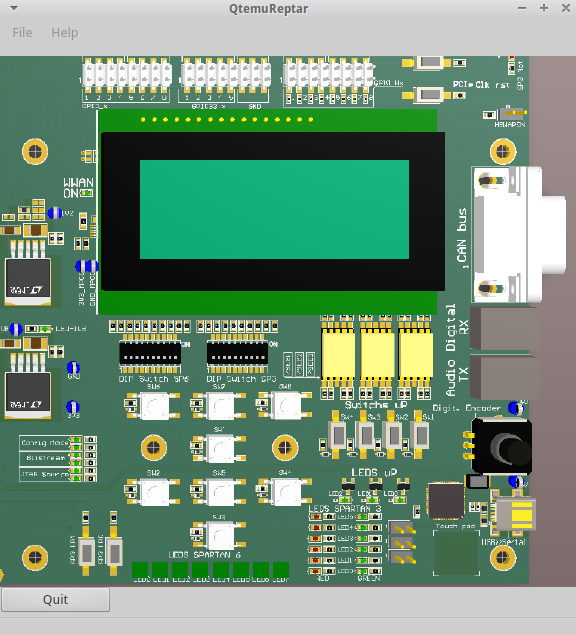
\includegraphics[width=10cm]{img/emulation1.png}
		\caption{Frontend graphique de Qemu}
		\label{emulation1}
	\end{center}
\end{figure}
\textbf{b) Donnée: }Les fichiers sources de Qemu se trouvent dans le répertoire qemu-reds. Examinez les fichiers
suivants :
\begin{enumerate}
	\item hw/arm/reptar/reptar.c Emulation plate-forme REPTAR
	\item hw/reptar\_sp6.c Emulation de la FPGA
	\item hw/reptar\_clcd.c Emulation gestion du LCD4x20
	\item hw/reptar\_sp6\_buttons.c Emulation gestion des boutons
	\item hw/reptar\_sp6\_emul.c Gateway entre Qemu et Qtemu
\end{enumerate}
Vous trouverez également toute la documentation nécessaire sur la plate-forme Reptar dans le
répertoire doc. \\\\
\textbf{Remarque: }Ces différents fichiers implémentent des modules noyaux.\\\\
\textbf{c) Donnée: } La compilation de Qemu pourra s'effectuer dans le répertoire qemu-reds directement, avec la
commande make (utilisez make -j4 ou -j8 pour aller plus vite !). \\\\
\textbf{Travail réalisé: }Par la suite, seule la commande \textit{make} sera nécessaire pour recompiler l'émulateur.\\
En lançant \textit{./qtemu} et Eclipse, on pourra debugger l'émulateur Qemu.
\begin{lstlisting}
redsuser@vm-reds-2015s2:~/seee_student$ cd qemu-reds/
redsuser@vm-reds-2015s2:~/seee_student/qemu-reds$ ./configure --target-list=arm-softmmu --enable-debug --disable-attr --disable-docs 
...
redsuser@vm-reds-2015s2:~/seee_student$ make -j8
...
redsuser@vm-reds-2015s2:~/seee_student$
\end{lstlisting}
\subsection{Émulation de la FPGA Spartan6}
Dans cette étape, il s'agit de mettre en place la structure nécessaire à l'émulation de la FPGA intégrée
à la plate-forme. La FPGA implémente des registres associés aux périphériques externes. Dans cette
étape, il s'agit de s'assurer que l'accès aux adresses I/O en lecture et écriture fonctionne. \\\\
\textbf{a) Donnée: }Complétez l'émulation de la FPGA afin de tester l'écriture et la lecture à l'une ou l'autre adresse
dédiée à la FPGA (affichez simplement un message). \\\\
\textbf{Travail réalisé: }Nous avons modifié les fichiers \textit{reptar\_sp6.c} et \textit{reptar.c}\\\\
\textbf{Emplacement du code:}\textit{/emulationSpartan6/reptar\_sp6.c} et \textit{/emulationSpartan6/reptar.c}\\\\
\textbf{b) Donnée: }Testez les accès en lecture-écriture avec U-Boot. \\\\
\textbf{Travail réalisé: }\\\\
\subsection{Émulation des devices de type LED (output)}

\subsection{Émulation de type boutons (input)}

\subsection{Gestion des interruptions (IRQ) avec les boutons}